\addchap{\Index{Programming guide}}

\chapter{\icewing{} Files} 

\section{Filesystem hierarchy}
\label{sec:p_filesystem}

Let's see, what the installation consists of. Below the
installation prefix, for example ``/usr/local'', you have this
structure-content:
\begin{description}
\item[bin/]
  \begin{description}
  \item \index{iceWing!icewing program}icewing - the executable itself
  \item \Index{icewing-config}

    A shell script similar to e.g. gtk-config which makes compiling
    of own plugins easy. It generates compiler-flags, extracts
    system-paths, and more. ``\verb|icewing-config --help|'' shows
    all available options of the script. See
    section~\ref{sec:icewing-config} for more details.
  \item \Index{icewing-docgen}

    A shell script which collects help messages of all plugins which
    are installed under \$\{PREFIX\}/lib/iceWing and all plugins which
    are integrated in \icewing{}. The script creates the files
    ``Readme.txt'' and ``Readme.html'' in the current directory and
    the file ``\$\{PREFIX\}/share/iceWing/plugins.help''. This last
    file is used by \icewing{} to display additional information
    about plugins on the ``Plugins'' page in the ``Plugin Info''
    window. See section~\ref{sub:PluginInfo} for information about
    this window. See section~\ref{sec:icewing-docgen} for more
    information about the script.
  \item \Index{icewing-plugingen}

    A plugin template generator. The script generates in the current
    directory a basic C or C++ plugin including a
    Makefile to compile it. ``\verb|icewing-plugingen --help|''
    gives more information. See section~\ref{sec:icewing-plugingen}
    for the details.
  \end{description}
  \verb|'icewing-config --bindir'| gives this directory,
  whereas \verb|'icewing-config --prefix'| gives the installation
  directory, i.e. this directory without the ``/bin'' part.
\item [include/] - All the headers for your own plugin programming
  \begin{description}
  \item iceWing - headers from the \icewing{} system

    Besides other options, \verb|'icewing-config --cflags'| contains
    this directory.
  \item iwPlugins - plugin headers

    If your plugin publishes new structures to be used by other
    plugins, you probably want to put them here.

    \verb|'icewing-config --pincludedir'| gives this directory.
  \end{description}
\item [lib/]
  \begin{description}
  \item iceWing/ - Here is the default place for \icewing{} to
    search for plugin libraries. Normally you give \icewing{} by
    command line parameter ``-l'' library names to load. If
    \icewing{} is not able to load them directly, it automatically
    tries to load them from this directory.

    \verb|'icewing-config --libdir'| gives this directory.
  \item pkgconfig/icewing.pc - A metadata file for
    \Index{pkg-config}, which can be used as an alternative to
    icewing-config for generating compiler-flags, extracting
    system-paths, and more. See section~\ref{sec:icewing-config} for
    more details.
  \end{description}
\item [man/] - The manpage of \icewing{}
\item [share/]
  \begin{description}
  \item iceWing/ - Place where \icewing{} and plugins can store
    additional data files. E.g. the plugin ``Face'' has here its
    config-file placed, and the polynom-classificator plugin stores
    its data here, too.
    \begin{description}
    \item \Index{icewing.pdf} - the manual of \icewing{}
    \item \Index{plugins.help} - This file is created by
      icewing-docgen. The file is used by \icewing{} to display
      additional information about plugins on the ``Plugins'' page
      in the ``Plugin Info'' window. See
      section~\ref{sub:PluginInfo} for information about this
      window.
    \end{description}

    \verb|'icewing-config --datadir'| gives this directory.
  \item log/icewing.log - The installation log file. It contains all
    actions performed during the ``make install'' phase.
  \end{description}
\end{description} 

%######################
\section{Headerfiles overview}
\label{sec:headerfiles}

TODO

%\chapter{General structure of a plugin}
%\section{Sources}
%\subsection{plugins/min/min.c}
%\subsection{plugins/min_cxx/min_cxx.cpp (Brief discussion: C vs C++)}
%\section{Compiling}
%First cd into the source-path of that plugin, check/edit the
%Makefile for e.g. correct ``FLAGS'' entry. Then compile the library
%with this commands:
%\sS
%\shellcom{make depend}
%\shellcom{make}
%\subsection{icewing-config}
%\subsection{Makefile for the ``typical plugin''}

\chapter{\icewing{} -- A CASE Tool}

\begin{quote}
  \textbf{Originally taken from \cite[Anhang B]{Loemker2004-LVO}.
    Since then translated by Ilker Savas and updated according to
    changes in \icewing{}.}
\end{quote}

\index{iceWing}
\label{chap:p_icewing}

During developing software in science there are certain extensive
tasks to do, which occur every time but do not belong to the real
task directly. Very often one needs a way to influence the
parameters of an algorithm easily and quickly. Similarly important
is the possibility to easily visualize any data. It must be easy to
examine and save the data at any time. In greater integrated systems
it is advantageous, if the different components can be developed
separately from each other without the loss of flexible and fast
interaction with each other afterwards.

In science an ergonomically sophisticated graphical user interface,
which can also be easily handled by a person not familiar with the
program, is mostly not needed. In most cases it is important that a
small team which is familiar with the task can easily develop and
optimize its special algorithm. This team of specialists must be
able to handle the user interface in an easy way. Thereby it is
mostly not intended to develop a complete program for an end
user. Several systems already offer functionality in these
directions. For example the commercial program
\matlab{}\index{Matlab} offers comprehensive options for
visualization and also for generation of graphical user interfaces,
which can be used easily via the provided scripting language
\cite{Matlab2003}. The open script language Tcl with its graphical
tool Tk\index{Tcl/Tk} offers also great facilities to generate user
interfaces \cite{Ousterhout1994-TAT}.

But existing systems usually are not optimized for the specific
needs during developing scientific software. \icewing{}, \emph{the
Integrated Communication Environment Which Is Not
Gesten}\footnote{This is a reference to an older program, the
predecessor of \icewing{}.} was developed to account for this
lack. \icewing{} is a graphical shell, which offers the above
mentioned functionalities to dynamically loadable
plugins\index{plugin} in an easy way. In the next sections
\icewing{} will be introduced more closely. First an overview of the
structure of plugins is given. The following chapters then give more
details of the various fields of \icewing{} in an exemplary
manner. So this is not a complete reference manual which would
describe all functions and types of \icewing{}. Further details not
mentioned here can be found in the header files and example plugins
of \icewing{}.

\section{Overview}
\label{sec:p_overview}

\begin{figure}[htb]
  \begin{center}
    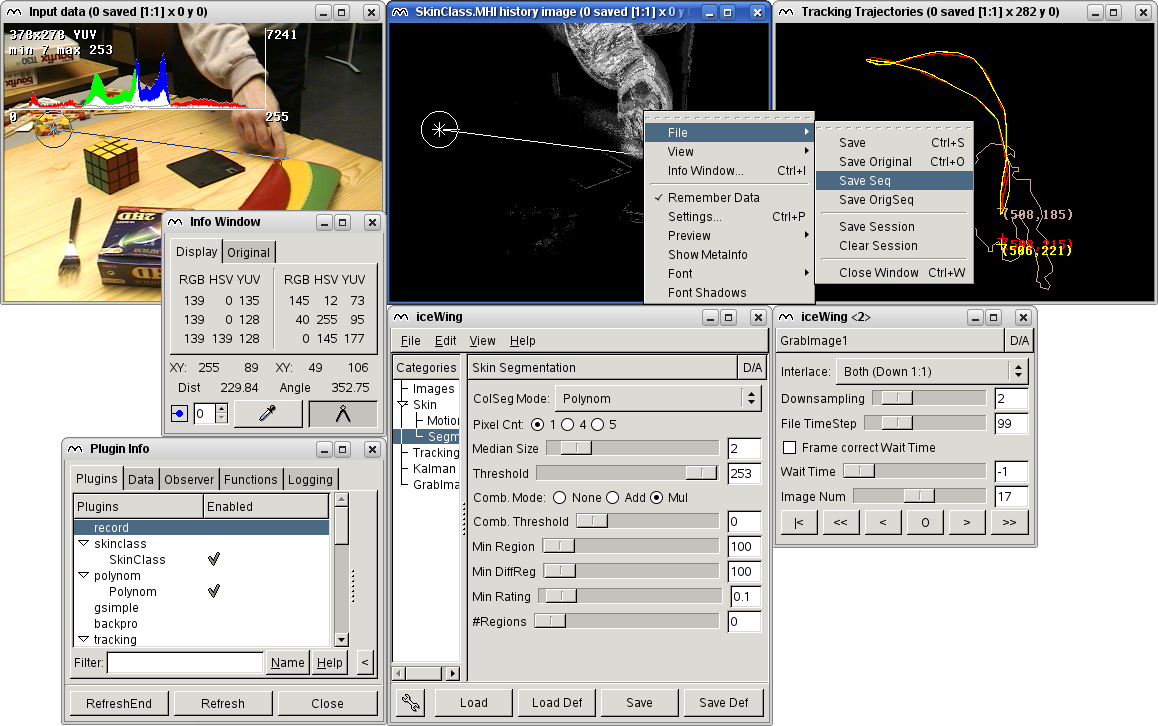
\includegraphics[width=\textwidth]{iw_main}
  \end{center}
  \caption[A typical session with \icewing{}]
  {A typical session with \icewing{}. Various intermediate
    results are being displayed and could be examined. Various
    parameters can be influenced interactively.}
  \label{fig:p_icewing}
\end{figure}

\icewing{} is a program written in the C language, which can
dynamically load plugins realized as shared libraries\index{shared
library}. It was tested on i386 Linux with the compilers GCC Version
2.95 up to Version 4.7\footnote{see http://gcc.gnu.org} and on
Alpha's with OSF 4.0f with the compilers DEC C Version 5.9 and GCC
Version 3.1. For graphical outputs as well as the user interface
generation the \Index{GTK} toolkit\footnote{see http://www.gtk.org}
Version 2.x or optionally Version 1.2 is used. With the help of
other external libraries the functionality can be extended, for
example towards supported graphical formats and supported cameras
for grabbing images. Figure~\ref{fig:p_icewing} demonstrates a
typical session with \icewing{} in which hands in a sequence of
images are segmented and tracked.

\paragraph{Plugins in \icewing{}}\hfill\\

\icewing{} the program only provides an initial user interface and
miscellaneous auxiliary routines. The real functionality is realized
by the various plugins that may be plugged into \icewing{}. Plugins
for \icewing{} must implement the interface shown in
Figure~\ref{fig:p_plugdef}. This is illustrated in
Figure~\ref{fig:p_min} with the help of a minimal plugin. The source
code of this plugin as well as a Makefile to compile it can be found
in the \icewing{} source distribution in the directory
``plugins/min/''\index{Plugin!min}. When the plugin, i.e. the shared
library, is first loaded, a function named
\fktIndex{plug$\_$get$\_$info()} is invoked. This is also the only
predetermined entry point in the library. This function is used to
create a new instance of the plugin -- it acts as a \Index{factory
function}. It returns a pointer to a filled structure of type
\typeIndex{plugDefinition}.

\begin{figure}[htb]
  \begin{center}
    \begin{small}
      \ovalbox{%
      \linespread{0.9}
\begin{BVerbatim}
typedef struct plugDefinition {
    char *name;
    int abi_version;
    void (*init) (struct plugDefinition *plug,
                  grabParameter *para, int argc, char **argv);
    int  (*init_options) (struct plugDefinition *plug);
    void (*cleanup) (struct plugDefinition *plug);
    BOOL (*process) (struct plugDefinition *plug,
                     char *id, struct plugData *data);
} plugDefinition;
\end{BVerbatim}%
      }
    \end{small}
  \end{center}
  \caption[The structure plugDefinition]
  {The structure plugDefinition, which every plugin must implement.}
  \label{fig:p_plugdef}
\end{figure}

The structure \type{plugDefinition} contains all the information
\icewing{} needs for a new plugin. The function pointers
\fkt{init()}, \fkt{init\_options()}, \fkt{cleanup()}, and
\fkt{process()} define entry points for the instance of the
plugin. \fkt{init()} is used for the general initialization of an
instance. For example it processes command line arguments for the
plugin instance. In \fkt{init\_options()} the graphical user
interface is initialized. More details about the user interface
initialization can be found in
section~\ref{sec:p_gui}. \fkt{cleanup()} is invoked at the end of
the program to release any resources. Finally \fkt{process()} is
called if the real functionality of the plugin is to be
executed. When this invocation happens can be determined with the
functions for the communication between plugins. For more details
see section~\ref{sec:p_kommunikation}. The variable \var{name}
declares the name of the instance. As the name serves as the
identification of the instance it must be unique among all loaded
plugins. \var{abi\_version} should always be set to the constant
\varIndex{PLUG\_ABI\_VERSION}. During runtime it is used to check if
the plugin was compiled against the correct \icewing{} version.

\begin{figure}[htb]
  \begin{center}
    \begin{small}
      \ovalbox{%
      \linespread{0.9}
\begin{BVerbatim}
#include "main/plugin.h"

static void min_init (plugDefinition *plug,
                      grabParameter *para, int argc, char **argv)
{
    ...
}

...

static plugDefinition plug_min = {
    "Min",
    PLUG_ABI_VERSION,
    min_init,
    min_init_options,
    min_cleanup,
    min_process
};

plugDefinition *plug_get_info (int cnt, BOOL *append)
{
    *append = TRUE;
    return &plug_min;
}
\end{BVerbatim}%
      }
    \end{small}
  \end{center}
  \caption[A minimal plugin]
  {The principal structure of a minimal plugin.}
  \label{fig:p_min}
\end{figure}

As the plugin in Figure~\ref{fig:p_min} always gives a fixed name
back it can be instantiated only one time. To change this the
structure of type \type{plugDefinition} has to be allocated
dynamically and the plugin name contained inside the structure must
be made unique for each invocation. This can be achieved by
integrating the instance number \var{cnt} into the name. \var{cnt}
contains the number of calls to the function
\fkt{plug\_get\_info()}. Thus \fkt{plug\_get\_info()} is modified
to:
\begin{small}
\linespread{0.9}
\begin{verbatim}
    *append = TRUE;
    plugDefinition *def = calloc (1, sizeof(plugDefinition));
    *def = plug_min;
    def->name = g_strdup_printf ("Min%d", cnt);
    return def;
\end{verbatim}
\end{small}
Now any number of instances of the plugin are possible.

Plugins in C++ can be realized in the same way as described above.
Alternatively one can use the C++ class shown in
figure~\ref{fig:p_cpp}. By deriving from this class the creation of
a plugin instance is also possible. In this case the factory
function \fkt{plug\_get\_info()} is modified to
\begin{small}
\linespread{0.9}
\begin{verbatim}
    *append = TRUE;
    ICEWING::Plugin* newPlugin =
            new ICEWING::MinPlugin (g_strdup_printf("C++Min%d", cnt));
    return newPlugin;
\end{verbatim}
\end{small}
where \type{ICEWING::MinPlugin} is a class derived from
\typeIndex{ICEWING::Plugin}. A C++ variant of the ``min'' plugin can
be found in the \icewing{} source distribution in the diretory
``plugins/min\_cxx/''\index{Plugin!min\_cxx}.

\begin{figure}[htb]
  \begin{center}
    \begin{small}
      \ovalbox{%
      \linespread{0.9}
\begin{BVerbatim}
namespace ICEWING {
    class Plugin : public plugDefinition {
    public:
        Plugin (char *name);
        virtual ~Plugin() {};

        virtual void Init (grabParameter *para, int argc, char **argv) = 0;
        virtual int  InitOptions () = 0;
        virtual bool Process (char *ident, plugData *data) = 0;
    };
}
\end{BVerbatim}%
      }
    \end{small}
  \end{center}
  \caption[The class Plugin]
  {The class Plugin, which allows the creation of plugins in C++ in
    a manner suitable for C++.}
  \label{fig:p_cpp}
\end{figure}

For simplified creation of new plugins a plugin generator is
available: \mbox{\emph{\Index{icewing-plugingen}}}.
icewing-plugingen is a shell script which expects up to three
arguments:
\sS
\shellcom{icewing-plugingen [-c|-cxx|-cpp] plugin-name short-name}
\sE
If ``-c'' is given, which is as well the default, a new C-plugin of
name ``plugin-name'' is generated in the current directory. If
``-cxx'' or ``-cpp'' is given, a C++-Plugin deriving from the class
Plugin is created. For the C-Version function and type names in the
generated source start with ``short-name''. Besides the needed
sources for the plugin a Makefile is generated and the plugin is
directly compiled for immediate testing. The plugin is kept short
and simple, but shows already data observation, easy user interface
generation, and rendering of data in a window.

\section{Communication between plugins}
\label{sec:p_kommunikation}

Within a main loop \icewing{} continuously invokes the loaded
plugins. The order of the invocation can be determined by the
plugins themselves. For this and for further communication of the
plugins \icewing{} offers several facilities. Plugins can exchange
data between each other. They can observe the storing of data by
other plugins and they can make functions available to other plugins
and invoke functions made available. Details about these
communication possibilities will now be given.

\paragraph{Data exchange}\hfill\\

In \icewing{} data consists of a string as an identifier, a
reference counter and a pointer to the concrete data. This data
element is deposited and made available for other plugins by the
function
\begin{small}
\linespread{0.9}
\begin{verbatim}
    typedef void (*plugDataDestroyFunc) (void *data);

    void plug_data_set (plugDefinition *plug, const char *ident,
                        void *data, plugDataDestroyFunc destroy);
\end{verbatim}
\fktindex{plug$\_$data$\_$set()}
\end{small}
The function \fkt{destroy()} is invoked when the reference counter
of the data has reached zero at the end of a main loop run. For
access to data provided by other plugins there are the functions
\begin{small}
\linespread{0.9}
\begin{verbatim}
    typedef struct plugData {
        plugDefinition *plug;   /* plugin which stored the data */
        char *ident;            /* ident under which the data was stored */
        void *data;             /* the stored data */
    } plugData;

    plugData* plug_data_get (const char *ident, plugData *data);
    plugData* plug_data_get_new (const char *ident, plugData *data);
    plugData* plug_data_get_full (const char *ident, plugData *data,
                                  BOOL onlynew, const char *plug_name);
\end{verbatim}
\typeindex{plugData}
\fktindex{plug$\_$data$\_$get()}
\fktindex{plug$\_$data$\_$get$\_$new()}
\fktindex{plug$\_$data$\_$get$\_$full()}
\end{small}
With \fkt{plug\_data\_set()} one can store several data elements
attached to one identifier. With the parameter \var{data} of
\fkt{plug\_data\_get()} one can access them successively. If the
value of this parameter is \var{NULL} then the data element first
stored under the identifier is returned. When invoked again with the
previously returned pointer the following data element is
returned. If \fkt{plug\_data\_get\_new()} is used only data elements
stored since the start of the current main loop run are
returned. Data elements stored during previous runs, which where not
freed because of increased reference counts, are skipped. If
\fkt{plug\_data\_get\_full()} is used, the returned data elements
can be additionally restricted to these elements, which were stored
by a special plugin.

Every invocation of \fkt{plug\_data\_get()} or one of its variants
increments the reference counter of the returned data
element. Increasing the reference counter of data, to which a
pointer is already available, can be done with the function
\begin{small}
\linespread{0.9}
\begin{verbatim}
    void plug_data_ref (plugData *data);
\end{verbatim}
\fktindex{plug$\_$data$\_$ref()}
\end{small}
The references can be released with the function
\begin{small}
\linespread{0.9}
\begin{verbatim}
    void plug_data_unget (plugData *data);
\end{verbatim}
\fktindex{plug$\_$data$\_$unget()}
\end{small}
Every successful call to \fkt{plug\_data\_get()} and every call to
\fkt{plug\_data\_ref()} requires a succeeding call to
\fkt{plug\_data\_unget()} to let the reference count drop
again. Finally this leads to an automatic call to the
\fkt{destroy()} function for releasing the data.

\paragraph{Observing data}\index{Observer}\label{para:observingData}\hfill\\

So far it is not clear when \icewing{} invokes the \fkt{process()}
functions of the plugins. This is determined by the observation of
data provided by other plugins. With the function
\begin{small}
\linespread{0.9}
\begin{verbatim}
    void plug_observ_data (plugDefinition *plug, const char *ident);
\end{verbatim}
\fktindex{plug$\_$observ$\_$data()}
\end{small}
a plugin can observe the storage of data with the identifier
\var{ident}. When \emph{new} data with this identifier gets stored,
the \fkt{process()} function of the observing plugin is invoked.

Data is considered new, if it is stored within the current main loop
run. At the start of a main loop run \icewing{} stores pseudo data
under the identifier \verb|"start"|. Every plugin that observes this
data will be invoked at the start of every main loop run. These
plugins can now store data themselves using their own identifiers to
initiate the call of other plugins observing these identifiers. If
there are no more plugins registered for the identifiers of newly
stored data, the next main loop run is initiated by again storing
pseudo data under the identifier \verb|"start"|. The different
plugins are invoked sequentially. Only if the \fkt{process()}
function of the previous plugin is finished the \fkt{process()}
function of the next plugin is invoked. Even if there were multiple
data elements stored under the same identifier the plugins are
normally invoked only once. Plugins that should process all data
elements stored under the same identifier must fetch them
sequentially with \fkt{plug\_data\_get()}.

This behavior can be changed with a special form for the variable
\var{ident}. If \verb|"ident()"| is given instead of \verb|"ident"|,
the plugin is invoked separately for all available data elements of
all plugins who's identifier the plugin is observing. When
\verb|"ident(plugin1 plugin2 ...)"| is given, the plugin is invoked
only for these plugins. The plugin is not invoked for data elements
from other plugins. This is done by using the functionality of the
function \fkt{plug\_add\_default\_page()}. See
page~\pagereftop{page:p_default_page} for more details. If the
function \fkt{plug\_add\_default\_page()} is called additionally,
any loaded default values for the plugin widget of
\fkt{plug\_add\_default\_page()} are ignored if \verb|"ident()"| or
\verb|"ident(plugin1 ...)"| is used here. I.e. the dependency
specifications from \fkt{plug\_observ\_data()} take precedence.

By invoking 
\begin{small}
\linespread{0.9}
\begin{verbatim}
    void plug_observ_data_remove (plugDefinition *plug, const char *ident);
\end{verbatim}
\fktindex{plug$\_$observ$\_$data$\_$remove()}
\end{small}
a plugin can stop its observation of data with a certain
identifier. Here, besides \verb|"ident"| \verb|"ident()"| and
\verb|"ident(plugin1 plugin2 ...)"| can be given for
\var{ident}. \verb|"ident"| only removes the
observer. \verb|"ident()"| removes the observer and any
dependent plugins in the widget from
\fkt{plug\_add\_default\_page()} or a previous call to
\fkt{plug\_observ\_data()} with a dependency
specification. \verb|"ident(plugin1 plugin2 ...)"| only removes the
specified plugins. Only if no dependent plugins for \verb|"ident"|
remain, the observer is removed as well.

\paragraph{Function exchange}\label{para:functionExchange}\hfill\\

The communication method described in the last paragraph is purely
data driven. Additionally there is the possibility for plugins to
provide their functions to other plugins. This can be achieved with
the function
\begin{small}
\linespread{0.9}
\begin{verbatim}
    typedef void (*plugFunc) ();

    void plug_function_register (plugDefinition *plug,
                                 const char *ident, plugFunc func);
\end{verbatim}
\fktindex{plug$\_$function$\_$register()}
\end{small}
Again with the help of the identifier \var{ident} a plugin can
access the registered function by means of the function
\begin{small}
\linespread{0.9}
\begin{verbatim}
    typedef struct plugDataFunc {
        plugDefinition *plug; /* plugin which registered the function */
        char *ident;          /* ident under which the function was registered */
        plugFunc func;        /* the registered function */
    } plugDataFunc;

    plugDataFunc* plug_function_get (const char *ident, plugDataFunc *func);
\end{verbatim}
\fktindex{plug$\_$function$\_$get()}
\end{small}
Similar to data storing many functions can be registered under the
same identifier. By setting \var{func} to \var{NULL} the first
function registered under an identifier can be accessed. Consecutive
calls to \fkt{plug\_function\_get()} with a previously returned
pointer yields the successively registered function. With the
function
\begin{small}
\linespread{0.9}
\begin{verbatim}
    void plug_function_unregister (plugDefinition *plug,
                                   const char *ident);
\end{verbatim}
\fktindex{plug$\_$function$\_$unregister()}
\end{small}
a provided function can be withdrawn by the plugin which provided
it. 

\section{Graphical abilities}
\label{sec:p_gui}

The graphical abilities of \icewing{} can be divided into three
groups. The first group incorporates functions for generating a
user interface consisting of widgets\index{widget}. The second group
contains functions for the display of various data. Furthermore
there are functions not classifiable into one of these groups
directly. The generation of the graphical interface mainly takes
place in the \fkt{init\_options()} function of each plugin. However,
every function described in this chapter can be invoked at any later
time as the user wishes. In the following sections these abilities
will be now introduced.

\subsection{Generating a user interface}
\label{sub:p_widgets}

Every widget that could be generated with \icewing{} functions
follows the same philosophy. During the generation of the widget the
address of a variable is passed to the generating function. This
variable is modified in the background by \icewing{}, without the
need of any help by the plugin. Indeed the plugin has no means to
modify the variable directly. Besides this, the screen layout for
the widgets is predetermined for the most part. This limitation
yields two benefits:
\begin{itemize}
\item The creation and management of widgets gets very simple for
  the plugins.
\item There is the possibility of automatically loading and saving
  widget values. This functionality is completely independent of any
  support coming from the plugin. Moreover, it is even possible to
  remotely set the widget values via \dacs{} again without the help
  of the plugin.
\end{itemize}
Figure~\ref{fig:p_widgets} gives an overview of all widget types
\icewing{} can create. The ``demo'' plugin, which was already used
during the quicktour (see section~\ref{sec:quicktour}), uses all
these widgets and additionally gives an overview over different
render capabilities of \icewing{}. It can be found in the \icewing{}
source distribution in the diretory ``plugins/demo/''\index{Plugin!demo}.

\begin{figure}[htb]
  \begin{center}
    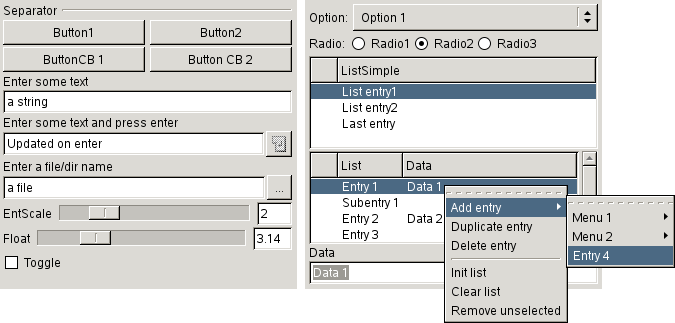
\includegraphics[width=12cm]{iw_widgets}
  \end{center}
  \caption[The widgets of \icewing{}]
  {All widgets \icewing{} provides for user interface generation.}
  \label{fig:p_widgets}
\end{figure}

\paragraph{Graphical user interface}\hfill\\

Widgets can be created on every page on the main window of
\icewing{}, in the context menu of display windows and in the
``Settings'' window of display windows. Figure~\ref{fig:p_icewing}
shows all these possible positions. A new page in the main window of
\icewing{} can be created with the function
\begin{small}
\linespread{0.9}
\begin{verbatim}
    int opts_page_append (const char *title);
\end{verbatim}
\fktindex{opts$\_$page$\_$append()}
\end{small}
\var{title} denotes the name to be displayed in the ``Categories''
list. If \var{title} contains a period or a space (\verb|"."|,
\verb|" "|), the ``Categories'' list will be displayed in a tree
structure. The return value of the function
\fkt{opts\_page\_append()} is an index that has to be specified
during the creation of a widget. The function
\begin{small}
\linespread{0.9}
\begin{verbatim}
    int prev_get_page (prevBuffer *b);
\end{verbatim}
\fktindex{prev$\_$get$\_$page()}
\end{small}
returns the index of the ``Settings'' window of display
windows. This enables the creation of widgets in these windows.

Widgets can be created with different functions for the different
widget types. The functions are all named according the pattern
\fkt{opts\_<widgetname>\_create()}. Examples of functions for four
different widget types are
\begin{small}
\linespread{0.9}
\begin{verbatim}
    void opts_separator_create (long page, const char *title);
    void opts_button_create (long page,
                             const char *title, const char *ttip,
                             gint *value);
    void opts_entscale_create (long page,
                               const char *title, const char *ttip,
                               gint *value, gint left, gint right);
    void opts_float_create (long page,
                            const char *title, const char *ttip,
                            gfloat *value, gfloat left, gfloat right);
\end{verbatim}
\fktindex{opts$\_$widgetname$\_$create()}
\end{small}
The parameter list of the functions again follows always the same
pattern. \var{page} denotes the page the widget should appear on. It
can be the return value of the function \fkt{opts\_page\_append()}
or \fkt{prev\_get\_page()}. Or, if the widget should be added to the
context menu of a display window, it is the pointer to the
corresponding \type{prevBuffer}. New widgets are always added at the
bottom of the specified page.

\var{title} denotes the name of the widget. In the examples in
figure~\ref{fig:p_widgets} it was for example
\verb|"Enter some text"| for the string widget and \verb|"EntScale"|
for the integer slider. This name together with the page name has to
be unique throughout the whole program as it is also used as the
identifier of the widget itself. The resulting identifier is
\verb|"pagetitle.widgettitle"|. With this identifier the widget is
addressable at any later time. Alternatively, to create the same
widget, \var{page} can be set to \var{-1} and \var{title} to the
complete identifier, i.e. \verb|"pagetitle.widgettitle"|.

If a widget with the identifier \verb|"pagetitle.widgettitle"|
already exists, the newly created widget replaces the old one. This
allows to change any widget parameter or even any widget type at any
time, for example the allowed range of values for a slider.

For entries in context menus of display windows submenus, default
hotkeys, and stock icons can be specified. For example, the
\var{title}
\verb|"Region/Draw white <<control>w> <stock gtk-select-color>"|
will create a menu entry ``Draw white'' in the submenu ``Region'',
which will have ``\textless{}control\textgreater{}w'' as its
hotkey and the stock icon ``gtk-select-color'' as its icon. The
hotkey can be later changed by the user by pressing the desired new
hotkey while the menu entry has the focus.

\var{ttip} specifies the tool tip of the widget. In \var{value} the
address of a variable has to be given. This variable is modified by
\icewing{} in the background in a dedicated thread. The plugin does
not need to care about querying the widget and setting the
variable. It can simply use the variable. The remaining parameters
specify the valid values of the variable \var{value}.

Additionally it is possible to set the value of a widget at a later
time and to delete a widget with the two functions 
\begin{small}
\linespread{0.9}
\begin{verbatim}
    long opts_value_set (const char *title, void *value);
    gboolean opts_widget_remove (const char *title);
\end{verbatim}
\fktindex{opts$\_$widget$\_$remove()}
\fktindex{opts$\_$value$\_$set()}
\end{small}
\var{title} denotes the identifier of a widget, i.e its page name
followed by a ``.'' and by the widget title. Additionally, the
\var{title} may contain the special characters '?' and '*'. If the
\var{title} can not be found directly and any of these characters
are inside the \var{title}, pattern matching is performed to find
the widget. Here '?' matches exactly one character and '*' matches
any number of characters. In case of an integer the value to be set
is passed directly in \var{value}, otherwise it is a pointer to the
value to be set. For example to set the value of the widget
\verb|"EntScale"| on page \verb|"demo"| in
figure~\ref{fig:p_widgets} to 3 one can use
\begin{small}
\linespread{0.9}
\begin{verbatim}
    opts_value_set ("demo.EntScale", GINT_TO_POINTER(3));
\end{verbatim}
\end{small}
whereas to set the \verb|"float"| widget
\begin{small}
\linespread{0.9}
\begin{verbatim}
    float newval = 3.0;
    opts_value_set ("demo.Float", &newval);
\end{verbatim}
\end{small}
must be used.

Sometimes it might be necessary to get the value of a widget where
one does not have direct access to. For this the function
\begin{small}
\linespread{0.9}
\begin{verbatim}
    void *opts_value_get (const char *title);
\end{verbatim}
\fktindex{opts$\_$value$\_$get()}
\end{small}
can be used, which returns a pointer to the current value from the
widget referenced by \var{title}. See \fkt{opts\_value\_set()} above
for more details about the \var{title}.

The current settings of all the different widgets created with one
of the \fkt{opts\_<widgetname>\_create()} functions can be loaded
and saved to/from files without any plugin interaction in the
graphical user interface. See paragraph~\ref{para:icewingValue} for
more details about these files. Sometimes it is desirable to not
load or save some of these settings. This can be achieved with the
functions
\label{page:p_defvalue_remove}
\begin{small}
\linespread{0.9}
\begin{verbatim}
    void opts_defvalue_remove (const char *title);
    void opts_save_remove (const char *title);
\end{verbatim}
\fktindex{opts$\_$defvalue$\_$remove()}
\fktindex{opts$\_$save$\_$remove()}
\end{small}
For both functions \var{title} denotes the identifier of the to be
affected widget. The function \fkt{opts\_defvalue\_remove()}
prevents, that settings from the configuration files, which are
automatically loaded during the start of \icewing{}, are applied to
the given widget. This function must be called before the
corresponding \fkt{opts\_<widgetname>\_create()} call. Otherwise the
settings were already applied. \fkt{opts\_save\_remove()} prevents
that the settings are saved to any configuration files in the first
place.

Normally, variables are simply modified by \icewing{} in the
background in a dedicated thread without any needed interaction of a
plugin. But \icewing{} can additionally call functions on value
change or when a different signal for a widget occurs. This is
achieved with the function
\begin{small}
\linespread{0.9}
\begin{verbatim}
    typedef struct optsWidget {
        char *title;       /* Full qualified name */
        char *wtitle;      /* Pointer inside title, widget name part */
        void *value;       /* Pointer to the widgets current value/variable */
    } optsWidget;

    typedef enum {
        OPTS_SIG_CHANGED = 1 << 0, /* The value of the widget has changed */
        OPTS_SIG_REMOVE  = 1 << 1  /* The widget is removed */
    } optsSignal;

    typedef void (*optsSignalFunc) (optsWidget *widget, void *newValue,
                                    void *data);

    gboolean opts_signal_connect (long page, const char *title,
                                  optsSignal sigset, optsSignalFunc cback,
                                  void *data);
\end{verbatim}
\typeindex{optsWidget}
\typeindex{optsSignal}
\typeindex{optsSignalFunc}
\fktindex{opts$\_$signal$\_$connect()}
\end{small}
The function \var{cback} is called with \var{data} as last argument
if one of the signals specified with \var{sigset} occurred for the
widget referenced by \var{title} and \var{page}. See
\fkt{opts\_<widgetname>\_create()} above for all the details about
\var{page} and \var{title}. If connecting \var{cback} was possible
\fkt{opts\_signal\_connect()} returns \var{TRUE}. Signal handlers
are invoked in the order they where connected.

For the list widget the signal \var{OPTS\_SIG\_CHANGED} is emitted
directly after changing the variable corresponding to the
widget. \var{newValue} is NULL in this case. For all other widgets
the signal \var{OPTS\_SIG\_CHANGED} is emitted just before the
variable corresponding to the widget is changed by
\icewing{}. \var{value} of \var{widget} still points to the old
value. \var{newValue} is a pointer to the new value for the
variable.

\paragraph{Nongraphical interface}\hfill\\

The automated treatment of variables of widgets for loading and
saving can be extended to variables that don't have a widget
assigned. This is provided by the functions
\begin{small}
\linespread{0.9}
\begin{verbatim}
    typedef enum {
        OPTS_BOOL, OPTS_INT, OPTS_LONG, OPTS_FLOAT, OPTS_DOUBLE, OPTS_STRING
    } optsType;

    typedef void (*optsSetFunc) (void *value, void *new_value, void *data);

    void opts_variable_add (const char *title,
                            optsSetFunc setval, void *data,
                            optsType type, void *value);
    void opts_varstring_add (const char *title,
                             optsSetFunc setval, void *data,
                             void *value, int length);
\end{verbatim}
\fktindex{opts$\_$variable$\_$add()}
\end{small}
\var{title} corresponds to the \var{title} variable of the widget
functions. \var{value} specifies the address of the variable to be
loaded and saved. With \var{type} their type is declared. If
\var{func} is set to \var{NULL} then in addition to be saved
automatically in the background the variable is also loaded and set
automatically. Otherwise the function \var{setval} with the
additional argument \var{data} gets invoked, if the variable should
be modified. This function is then responsible for the modification
of the variable. With the function \fkt{opts\_varstring\_add()} one
can additionally specify a maximal length for a string, which will
be not exceeded during the setting of the string.

\paragraph{Plugin support}\label{para:pluginSupport}\hfill\\

There are certain standardized functions which are (a) controllable
by widgets and (b) interesting for a lot of plugins. In addition
most plugins need at least one page to place their widgets on. To
simplify this there is the following function which creates a new
page with two special widgets:
\label{page:p_default_page}
\begin{small}
\linespread{0.9}
\begin{verbatim}
    typedef enum {
        PLUG_PAGE_NOPLUG        = 1 << 0,
        PLUG_PAGE_NODISABLE     = 1 << 1
    } plugPageFlags;

    int plug_add_default_page (plugDefinition *plugDef,
                               const char *suffix,
                               plugPageFlags flags);
\end{verbatim}
\typeindex{PLUG$\_$PAGE$\_$NOPLUG}
\typeindex{PLUG$\_$PAGE$\_$NODISABLE}
\fktindex{plug$\_$add$\_$default$\_$page()}
\end{small}
This function creates a new page in the main window of \icewing{}
under the name '\var{plugDef->name}\verb|" "|\var{suffix}' and
returns its index. Furthermore up to two widgets are created whose
functionalities are completely realized by \icewing{}. The first
widget toggles the invocation of the \fkt{process()} function of the
plugin. If \type{PLUG\_PAGE\_NODISABLE} is given in \var{flags},
this widget is suppressed.

The second widget is created if \type{PLUG\_PAGE\_NOPLUG} is not set
in \var{flags}. With this widget one can control which data elements
of which other plugins should be passed to the plugin
\var{plugDef}. Normally the function \fkt{process()} of the plugin
\var{plugDef} is invoked as soon as data with an identifier observed
by \var{plugDef} is provided by any other plugin. Even though there
could be more than one data element available under the observed
identifier at the time the plugin is invoked only once. The plugin
can get the remaining data elements by using the function
\fkt{plug\_data\_get()}.

With the function \fkt{plug\_add\_default\_page()} this behavior is
changed. If in this case nothing is entered in the second widget,
the plugin is invoked separately for all available data elements of
all plugins, who's identifier the plugin is observing. When there are
names of plugins in the widget, the plugin is invoked only for these
plugins. The plugin is not invoked for data elements from other
plugins.

Since this widget supplies \icewing{} with additional information
about the interdependencies between the registered plugins, the
order of invocation of the plugins can be changed accordingly if
necessary. If multiple plugins observe the same identifier
\verb|"ident"| normally the order of their invocation is not
determined. However, if in one plugin's
\fkt{plug\_add\_default\_page()} widget is specified that the plugin
want's to get \verb|"ident"| from one of these other plugins, then
this other plugin is always invoked first. As an example suppose
that plugins ``A'' and ``B'' both observe \verb|"image"|. If now the
user specified in the widget of plugin ``A'' that ``A'' should get
\verb|"image"| from plugin ``B'', plugin ``B'' is always invoked
before plugin ``A'' if data of type \verb|"image"| is available.

For easy creation of names of the form
'\var{plugDef->name}''\var{suffix}' 
there is the function
\begin{small}
\linespread{0.9}
\begin{verbatim}
    int plug_name (plugDefinition *plugDef, const char *suffix);
\end{verbatim}
\fktindex{plug$\_$name()}
\end{small}
which returns a pointer to a per-plugin-instance string of the
form '\var{plugDef->name}''\var{suffix}'. This often comes handy for
accessing widgets on the page created for example by
\fkt{plug\_add\_default\_page()} but as well to create pages with
\fkt{opts\_page\_append()} or to access widgets on these pages. All
widget names in \icewing{} have to be unique. If these pages use
this naming scheme as well, the names are easily made unique. The
same is true for the function \fkt{prev\_new\_window()}, where this
nameing scheme should be used as well.

Sometimes, plugins need to store additional data files. The
function
\begin{small}
\linespread{0.9}
\begin{verbatim}
    char *plug_get_datadir (plugDefinition *plug);
\end{verbatim}
\fktindex{plug$\_$get$\_$datadir()}
\end{small}
returns an appropriate path where \var{plug} can store its data
files. If the library the plugin was instantiated from was loaded
from its default path, the function returns
\$\{PREFIX\}/share/iceWing, if it was loaded from the \icewing{} path
in the users home directory \urltilde{}/.icewing/data is
returned, and if the lib was loaded from one of the
\Index{ICEWING\_PLUGIN\_PATH} directories
\$\{ICEWING\_PLUGIN\_PATH\}/data is returned. See
page~\pagereftop{page:opt_l_libs} as well for the \icewing{} command
line option ``-l'', which loads plugin libraries.

\subsection{Graphical display of data}
\label{sub:p_rendering}

\icewing{} offers various possibilities for data
visualization. Plugins can create any number of data display
windows. The user may at any time open and close these windows,
scroll and zoom in them, save their contents or display meta
informations about their content. During these actions vector
objects like lines and ellipses get correctly redrawn at the desired
zoom level. All these actions do not involve the plugins, since the
display windows are managed completely by \icewing{}.

\paragraph{Window management}\hfill\\

New windows can be created by the function
\begin{small}
\linespread{0.9}
\begin{verbatim}
    typedef struct prevBuffer {
        ...
        guchar *buffer;       /* buffer for the image */
        int width, height;    /* width, height of the buffer */
        GtkWidget *window;    /* window in which the buffer is displayed */
        ...
    } prevBuffer;

    prevBuffer *prev_new_window (const char *title, int width, int height,
                                 gboolean gray, gboolean show);
\end{verbatim}
\typeindex{prevBuffer}
\fktindex{prev$\_$new$\_$window()}
\end{small}
\var{title} is on the one hand the name of the window and on the
other hand an identifier. This identifier together with the names of
the pages created with \fkt{opts\_page\_append()} in the \icewing{}
main window has to be unique throughout the whole program. If the
name contains a period (\verb|"."|) the windows in the ``Images''
list in the main window will be displayed in a tree
structure. \var{width} and \var{height} specify the initial size of
the window. The user can resize the window at any time. Specifying
\var{-1} means that the default values for width and height are
taken. \var{gray} determines if the content of the window is
displayed in gray or in color. If \var{show = TRUE} the window is
opened instantly after creation. Otherwise the user has to
double-click on the window title in the ``Images'' list to open the
window.

Bigger amounts of memory are used not before the window is opened
the first time. Every drawing function of \icewing{} first tests if
a window is actually open before drawing and returns immediately if
this is not the case. So the consumption of computer resources stays
low even if many windows are created and outputs in them are
produced without any further checks. Sometimes it is useful to check
whether a window is open before any complex computations of output
data for the window is carried out. This can be done with
\verb|(buffer->window != NULL)|. With
\begin{small}
\linespread{0.9}
\begin{verbatim}
    void prev_free_window (prevBuffer *b);
\end{verbatim}
\fktindex{prev$\_$free$\_$window()}
\end{small}
one can remove and free a window previously created with
\fkt{prev\_new\_window()}.

The user can scroll and zoom in the windows at any
time. Additionally these actions can be performed by the plugin
using the function
\begin{small}
\linespread{0.9}
\begin{verbatim}
    void prev_pan_zoom (prevBuffer *b, int x, int y, float zoom);
\end{verbatim}
\fktindex{prev$\_$pan$\_$zoom()}
\end{small}
The content of window \var{b} is then displayed at location
\var{(x,y)} with a zoom value of \var{zoom}. If any of the
parameters are below zero, the respective old values are retained.

Some plugins need informations about mouse actions and key presses
in a particular window. They can be retrieved with the functions
\begin{small}
\linespread{0.9}
\begin{verbatim}
    typedef enum {
        PREV_BUTTON_PRESS               = 1 << 0,
        PREV_BUTTON_RELEASE             = 1 << 1,
        PREV_BUTTON_MOTION              = 1 << 2
        PREV_KEY_PRESS                  = 1 << 3,
        PREV_KEY_RELEASE                = 1 << 4
    } prevEvent;
    typedef void (*prevButtonFunc) (prevBuffer *b, prevEvent signal,
                                    int x, int y, void *data);
    typedef void (*prevSignalFunc) (prevBuffer *b, prevEventData *event,
                                    void *data);

    void prev_signal_connect (prevBuffer *b, prevEvent sigset,
                              prevButtonFunc cback, void *data);
    void prev_signal_connect2 (prevBuffer *b, prevEvent sigset,
                               prevSignalFunc cback, void *data);
\end{verbatim}
\fktindex{prev$\_$signal$\_$connect()}
\fktindex{prev$\_$signal$\_$connect2()}
\end{small}
If one of the events specified by \var{sigset} occurs, which is
triggered by a mouse button or a key press in window \var{b}, the
function \fkt{cback()} with the additional argument \var{data} is
invoked. \fkt{cback()} is additionally provided with the event
occurred and further information about the event. The function
\fkt{prev\_signal\_connect()} only enables the handling of mouse
events whereas \fkt{prev\_signal\_connect2()} permits the handling
of both mouse events as well as key press events. The effects of
zooming and scrolling are completely removed from the passed mouse
coordinates.

\paragraph{The display of graphical objects}\hfill\\

\begin{figure}[htb]
  \begin{center}
    \includegraphics[width=\textwidth]{iw_render}
  \end{center}
  \caption[\icewing{}'s graphical elements]
  {All graphical elements \icewing{} can render.}
  \label{fig:p_render}
\end{figure}

\icewing{} provides the possibility to display miscellaneous
graphical primitives in the windows created by
\fkt{prev\_new\_window()}. Figure~\ref{fig:p_render} gives a
summary of all primitives \icewing{} can create. The display of the
objects is accomplished in multiple stages. The first step is
optional and, if enabled, copies all of the original data which is
needed for the display of an object. With this data \icewing{} can
redraw the image without interaction with the plugin -- scrolling
and zooming in high quality gets possible without the plugins
help. Subsequently the objects are displayed in an off-screen buffer
using the current scroll and zoom values. This buffer contains the
precise section of the image which will be seen in the window and
hence can be used for redrawing the window - again without the
involvement of the plugin. In a final step the buffer is then drawn
into the window.

All objects can be displayed using different functions with a common
interface. Two examples of these functions are
\begin{small}
\linespread{0.9}
\begin{verbatim}
    typedef enum {
        PREV_IMAGE,
        PREV_TEXT,
        PREV_LINE,
        ...
        PREV_NEW = 30
    } prevType;

    #define RENDER_THICK    (1<<30)  /* use thickness for vector objects */
    #define RENDER_CLEAR    (1<<31)  /* clear the buffer and free all old render
                                        data (IMPORTANT to prevent mem leaks) */

    void prev_render_data (prevBuffer *b, prevType type, const void *data,
                           int disp_mode, int width, int height);
    void prev_render_list (prevBuffer *b, prevType type, const void *data,
                           int size, int cnt,
                           int disp_mode, int width, int height);
\end{verbatim}
\typeindex{prevType}
\fktindex{prev$\_$render$\_$data()}
\fktindex{prev$\_$render$\_$list()}
\varindex{RENDER$\_$THICK}
\varindex{RENDER$\_$CLEAR}
\end{small}
Every render function gets different standard arguments. Window
\var{b} is the window in which the object is displayed. With
\var{width} and \var{height} one can specify the total size of all
objects which are still inside the window. These latter two values
are needed to compute the correct zoom factor for the display of the
object if the ``Fit to window'' display mode for the window is
chosen. If these values are -1 or \var{RENDER\_CLEAR} is \emph{not}
set in \var{disp\_mode}, the last values for the buffer
\var{b} are used instead. With \var{disp\_mode} the rendering can be
influenced. If \var{RENDER\_CLEAR} is specified the contents of the
whole window is cleared and the internal copies of all parameters of
former drawing actions are freed before drawing. \var{RENDER\_THICK}
enables the rendering of thicker lines by means of a special
setting. See the function \fkt{prev\_set\_thickness()} for more
details. The remaining arguments specify the particular object,
which should be displayed in the window. With
\fkt{prev\_render\_data()} an arbitrary object can be displayed and
\fkt{prev\_render\_list()} displays an array of objects of the same
type. \var{type} specifies the type of the objects. \var{data} is in
the first case a pointer to the data of one object and in the second
case a pointer to the data of an array of objects. In the second
case \var{cnt} gives the length of the array and \var{size} denotes
the size of an array element.

Data for objects to be displayed must be specified via
structures. For example for lines it is
\begin{small}
\linespread{0.9}
\begin{verbatim}
    typedef struct {
        iwColtab ctab;
        int r, g, b;
        int x1, y1, x2, y2;
    } prevDataLine;
\end{verbatim}
\typeindex{prevDataLine}
\end{small}
The structures for the other available objects are similar. \var{ctab}
determines how \var{r}, \var{g} and \var{b} should be
interpreted. For example if \var{ctab} is set to \var{IW\_RGB} then
they are interpreted as a point in the RGB color space, with
\var{IW\_YUV} as a point in the YUV color space, or with a pointer
to a color table \var{r} would be interpreted as an index in this
color table. Specifying \var{-1} for \var{r}, \var{g}, or \var{b} has
a special meaning. In this case the corresponding color channel is not
modified during the rendering. Finally \var{x1}, \var{y1}, \var{x2}
and \var{y2} are the coordinates of the endpoints of the line. To
enable subpixel accurate displaying of objects there are \var{float}
data type variants of every vector object structure, for
example \typeIndex{prevDataLineF} for lines. For displaying these
data elements there are corresponding prevType values like
\var{PREV\_LINE\_F} for lines.

To simplify the call to \fkt{prev\_render\_list()} there is a
wrapper for every object type. For example arrays of lines or images
can be displayed also using the functions
\begin{small}
\linespread{0.9}
\begin{verbatim}
    void prev_render_lines (prevBuffer *b,
                            const prevDataLine *lines, int cnt,
                            int disp_mode, int width, int height);
    void prev_render_imgs (prevBuffer *b,
                           const prevDataImage *imgs, int cnt,
                           int disp_mode, int width, int height);
\end{verbatim}
\fktindex{prev$\_$render$\_$lines()}
\fktindex{prev$\_$render$\_$imgs()}
\end{small}
In image processing very often one needs to display an image. For
the frequent case of 8 bit images there is the function
\begin{small}
\linespread{0.9}
\begin{verbatim}
    void prev_render (prevBuffer *b, guchar **planes,
                      int width, int height, iwColtab ctab);
\end{verbatim}
\fktindex{prev$\_$render()}
\end{small}
with which no structure has to be filled in this case. Additionally
by setting \var{RENDER\_CLEAR} this function clears the complete
window before rendering the image. To render other types of images
-- \icewing{} also supports images of type 16 bit int, 32 bit int,
float, and double -- or to support other forms of flexibility
the previously introduced function \fkt{prev\_render\_imgs()} or
the different general render functions must be used.

For simplified text output there is additionally the function
\begin{small}
\linespread{0.9}
\begin{verbatim}
    void prev_render_text (prevBuffer *b,
                           int disp_mode, int width, int height,
                           int x, int y, const char *format, ...);
\end{verbatim}
\fktindex{prev$\_$render$\_$text()}
\end{small}
This function invokes \fkt{sprintf()} internally and and renders
the returned string. The string can contain additional
formatting instructions to modify color, type and alignment
of the rendering. For example by embedding
\verb|<fg="255 0 0" bg="0 0 0" font=big>| it can be switched to a
big red font on a black background. Further details about the
formatting instructions can be found in the header ``Grender.h''.

The rendering of objects can be influenced further by the two
functions:
\begin{small}
\linespread{0.9}
\begin{verbatim}
    void prev_set_bg_color (prevBuffer *buf, uchar r, uchar g, uchar b);
    void prev_set_thickness (prevBuffer *buf, int thickness);
\end{verbatim}
\fktindex{prev$\_$set$\_$bg$\_$color()}
\fktindex{prev$\_$set$\_$thickness()}
\end{small}
\fkt{prev\_set\_bg\_color()} determines with which color the window
is cleared if \var{RENDER\_CLEAR} is set. With
\fkt{prev\_set\_thickness()} lines are drawn with the specified
thickness if \var{RENDER\_THICK} was set during the output of
objects.

All functions for drawing objects introduced so far draw the objects
incrementally in an off-screen buffer assigned to the appropriate
window. In a final step this buffer can be rendered in the
associated window using the function
\begin{small}
\linespread{0.9}
\fktindex{prev$\_$draw$\_$buffer()}
\begin{verbatim}
    void prev_draw_buffer (prevBuffer *b);
\end{verbatim}
\end{small}
The steps to follow to render something in a window using \icewing{}
can be summarized as:
\begin{equation*}
  \parbox{14.5cm}{\begin{struktogramm}{14.5cm}{0.4cm}
      \BLOCK{Create a new window \var{b} with
        \fkt{prev\_new\_window()}. This is the necessary first step and
        can be well placed in the \fkt{init\_options()} function of the
        plugin. But any later executed code paths are as well possible.}
      \LOOP{
        \BLOCK{Render various objects in the off-screen buffer of
          window \var{b} using several of the
          \fkt{prev\_render\_xxx()} functions. \var{RENDER\_CLEAR}
          must be set before the first function is invoked to clear
          the window beforehand.}
        \BLOCK{Render the off-screen buffer in window \var{b} by
          invoking the function \fkt{prev\_draw\_buffer()}.}
      }
    \end{struktogramm}}
\end{equation*}
Besides this described interface with the \fkt{prev\_render\_xxx()}
functions to render objects there is also another interface
consisting of \fkt{prev\_drawXxx()} functions. This is an interface
with lower abstraction which for example ignores scroll positions as
well as zoom adjustments. Because of this it should not be used most
of the time. If this low level interface is necessary nevertheless,
further details about its usage can be found in the according
header files.

\subsection{Further graphical functionalities}

If the program has to be terminated this should never be managed
using the regular ANSI function \fkt{exit()}. For this one should
always use the function
\begin{small}
\linespread{0.9}
\begin{verbatim}
    void gui_exit (int status);
\end{verbatim}
\fktindex{gui$\_$exit()}
\end{small}
The direct call to \fkt{exit()} can lead to a segmentation violation
as well as to a freeze of the complete program. As various graphical
abilities are realized in a dedicated seperate thread, an accurate
synchronization with this thread has to be performed before
termination. This synchronization is ensured by \fkt{gui\_exit()}.

In \icewing{} images are managed by the structure
\begin{small}
\linespread{0.9}
\begin{verbatim}
    typedef enum {
        IW_8U, IW_16U, IW_32S, IW_FLOAT, IW_DOUBLE
    } iwType;

    typedef struct iwImage {
        guchar **data;      /* the real image data */
        int planes;         /* number of planes available in data */
        iwType type;        /* type of data */
        int width, height;  /* width, height of the image in pixel */
        int rowstride;      /* distance in bytes between two lines */
                            /* if >0: color images are interleaved in data[0] */
        iwColtab ctab;      /* color space used in data */
    } iwImage;
\end{verbatim}
\typeindex{iwType}
\typeindex{iwImage}
\end{small}
In this structure image data can be stored in various types and
arrangements. With \type{iwType} the type of \var{data} is
specified ranging from 8 bit unsigned to double. The arrangement of
the image data can be \emph{planed} as well as
\emph{interleaved}. In a planed arrangement the color planes are
provided separately in the fields \var{data[0]}, \var{data[1]},
\dots, \var{data[planes-1]}. In an interleaved arrangement
\var{data[0]} contains all the color information where the
particular color values of a pixel are juxtaposed in the array. For
example for \var{planes=3} in the RGB color space first the red
color value of the first pixel is stored followed by the green and
blue values. Subsequently the values of the second pixel are stored
in the same way until finally the values of pixel \var{width*height}
are reached and stored in \var{data[0]}. Images of all these types
and arrangements can be created, released, loaded, saved, and also
displayed.

There are several functions for managing images of which some of the
important ones are:
\begin{small}
\linespread{0.9}
\begin{verbatim}
    gboolean iw_img_allocate (iwImage *img);
    iwImage* iw_img_new (void);
    iwImage* iw_img_new_alloc (int width, int height,
                               int planes, iwType type);
    void     iw_img_free (iwImage *img, iwImgFree what);
    iwImage* iw_img_load (const char *fname, iwImgStatus *status);
    iwImgStatus iw_img_save (const iwImage *img, iwImgFormat format,
                             const char *fname, const iwImgFileData *data);
\end{verbatim}
\fktindex{iw$\_$img$\_$allocate()}
\fktindex{iw$\_$img$\_$new()}
\fktindex{iw$\_$img$\_$new$\_$alloc()}
\fktindex{iw$\_$img$\_$free()}
\fktindex{iw$\_$img$\_$load()}
\fktindex{iw$\_$img$\_$save$\_$format()}
\end{small}
Further details about these and several other functions for managing
images can be found in the header file ``\Index{Gimage.h}''.

\section{Further abilities}

Besides the so far explained abilities \icewing{} has further
functionalities in the graphics as well as in some other areas. In
this section some of them will be introduced more closely where some
others will not be detailed much. For example in the header file
``output.h'' there are functions to ease the use of \dacs{}. These
include functions for image output, for the output of status
messages and for the output of general data via
streams. Furthermore, it is possible to make functions available for
RPC communication via \dacs{}. All these functions manage the
registration with \dacs{}, the error handling and the generation of
unique stream names and function names.

Further examples of useful functions include ``session management'' or
functions that allow the registration of new graphical primitives
that can then be used with the general rendering functions. Further
details of these as well as the so far presented functions can be found in
the appropriate header files of \icewing{}.

\subsection{The ``grab'' plugin}
\index{Plugin!grab}

A central plugin is the in \icewing{} integrated plugin ``grab''. It
enables the import and the delivering of a series of images for
further processing to other plugins. The images can be imported from
a grabber (controlled by various drivers, e.g Video4Linux or
FireWire), from \dacs{} encoded in the \type{Bild\_t}
format, or from files of various pixel formats. Once ``grab'' is
invoked by \icewing{} it imports the next image and makes it
available for other plugins under the ident ``image'' using the
function \fkt{plug\_data\_set()}. For the image the YUV color space
is used. The structure that ``grab'' uses to provide the data is
derived from iwImage, i.e. it first contains the image and
afterwards different additional data. In detail, the structure is:
\label{page:p_grabImageData}
\begin{small}
\linespread{0.9}
\begin{verbatim}
    typedef struct grabImageData {
        iwImage img;         /* the image data */
        struct timeval time; /* time the image was grabbed */
        int img_number;      /* consecutive number of the grabbed image */
        char *fname;         /* image read from a file? -> name of the file */
        int frame_number;    /* image from video file -> frame number, else 0 */
        float downw, downh;  /* down sampling, which was applied to the image */
    } grabImageData;
\end{verbatim}
\typeindex{grabImageData}
\end{small}
The image is allways encoded in the planed format, i.e. the color
planes are provided separately in the fields \var{data[0]},
\var{data[1]}, \dots, \var{data[planes-1]} of the \type{iwImage}
structure. Additionally the plugin can provide the imported images
via a \dacs{} stream in the \type{Bild\_t} format. By means of a
\dacs{}-function the current or optionally also past images can be
fetched from other programs in the \type{Bild\_t} format.

If there is an observer for the identifier \verb|''imageRGB''|, then
additionally the current image is provided in the RGB color space
under this identifier using the function
\fkt{plug\_data\_set()}. For the storing of the data associated with
``imageRGB'' again the \type{grabImageData} structure is used.

\paragraph{Changing grabber arguments}\hfill\\

When a grabber is used to access the images, e.g. when the grabbing
plugin was started with the option ``-sg'', it is possible for every
plugin to change at any time various parameters of the grabbing
process. There are two possibilities to achieve this. The first
option is to completely restart the grabbing process by changing the
arguments, which where initially supplied to the ``-sg''
option. With this approach everything from
section~\ref{sec:para_driver} can be specified and/or changed. This
approach uses the GUI widget described in paragraph
\ref{para:grabOptions} to provide the options to the grabbing
driver:
\begin{small}
\linespread{0.9}
\begin{verbatim}
    char *old = opts_value_get ("GrabImage1.Grabbing driver options:");
    char str[500];
    sprintf (str, "bayer=bilinear:%s", old);
    opts_value_set ("GrabImage1.Grabbing driver options:", str);
\end{verbatim}
\index{Grabbing driver options}
\end{small}
In this example the bayer argument is added to the first instance of
the grabber plugin. If the bayer argument was specified previously,
it is automatically removed on reinit of the grabbing process. If
arguments are identical only the initial ones remain.

The second option allows to change single arguments on the fly,
i.e. without a restart of the grabbing process. The disadvantage of
this approach is that only some arguments of the grabbing plugin
can be changed this way as the different grabbing drivers need
special support for every argument. During initialization the
grabbing plugin provides a function ``setProperties'' via
\fkt{plug\_function\_register()} (see paragraph
\ref{para:functionExchange} for details about function exchange
between plugins), which can be used to get or set different
arguments at the same time. Here is an example which changes some
arguments and prints the names of all properties of the current
driver:
\begin{small}
\linespread{0.9}
\begin{verbatim}
    #include "main/grab_prop.h"

    plugDataFunc *propFunc;
    iwGrabProperty *props;

    propFunc = plug_function_get (IW_GRAB_IDENT_PROPERTIES, NULL);
    ((iwGrabPropertiesFunc)propFunc->func) (propFunc->plug,
                              IW_GRAB_SET_ROI, 11,12,13,14,
                              IW_GRAB_SET_PROP, "propGain=0.3:prop4=0.7",
                              IW_GRAB_LAST);
    ((iwGrabPropertiesFunc)propFunc->func) (propFunc->plug,
                              IW_GRAB_GET_PROPVALUES, &props,
                              IW_GRAB_LAST);
    if (props)
        for (int i=0; props[i].name; i++)
            printf("%d: %s\n", i, props[i].name);
\end{verbatim}
\end{small}
The header ``grab\_prop.h'' contains all the details and more
documentation about this approach.

\subsection{Auxiliary functions}

``\Index{tools.h}'' provides several smaller auxiliary routines that
are frequently needed during program development. These include
functions for the output of errors, warnings, debug messages and
functions for testing assertions:
\begin{small}
\linespread{0.9}
\begin{verbatim}
    void iw_debug (int level, const char *str, ...);
    void iw_debug_1 (int level, const char *str);
    void iw_debug_2 (int level, const char *str, ARG1);
    ...
    void iw_warning (const char *str, ...);
    void iw_warning_1 (const char *str);
    void iw_warning_2 (const char *str, ARG1);
    ...
    void iw_error (const char *str, ...);
    void iw_error_1 (const char *str);
    void iw_error_2 (const char *str, ARG1);
    ...
    void iw_assert (scalar expression, const char *str, ...);
    void iw_assert_1 (scalar expression, const char *str);
    void iw_assert_2 (scalar expression, const char *str, ARG1);
    ...
\end{verbatim}
\end{small}
All these functions invoke \fkt{sprintf()} internally. The functions
\fktIndex{iw$\_$debug$\_$xxx()} and \fktIndex{assert$\_$xxx()} only
produce code if the macro \varIndex{IW\_DEBUG} is set during
compilation. \fkt{iw\_debug\_xxx()} only produces output if the
value of \var{level} is smaller than \var{talklevel} which can be
chosen via the command line of \icewing{} (option ``-t'', see
page~\pagereftop{page:opt_t_talk}). \fktIndex{iw$\_$warning$\_$xxx()}
always outputs its message, whereas \fktIndex{iw$\_$error$\_$xxx()}
additionally terminates the execution of the program. The function
variants without a number, i.e. \fkt{iw\_debug()},
\fkt{iw\_warning()}, \fkt{iw\_error()}, and \fkt{iw\_assert()},
allow an arbitrary number of arguments, but for full functionality
they need either GCC or another compiler compatible with
ANSI-C99. Otherwise these variants are implemented as functions
instead of macros, which provide less information than the macro
variants.

Additionally there are several functions for meassuring the
execution time of program parts. Some of them are:
\begin{small}
\linespread{0.9}
\begin{verbatim}
    int  iw_time_add (const char *name);
    void iw_time_start (int nr);
    long iw_time_stop (int nr, BOOL show);

    #define iw_time_add_static(number,name) ...
    #define iw_time_add_static2(number,name,number2,name2) ...
\end{verbatim}
\fktindex{iw$\_$time$\_$add()}
\fktindex{iw$\_$time$\_$start()}
\fktindex{iw$\_$time$\_$stop()}
\fktindex{iw$\_$time$\_$add$\_$static()}
\end{small}
\fkt{iw\_time\_add()} creates a new timer and returns an index to
it. Using this index it can be started with the function
\fkt{iw\_time\_start()} and stopped with
\fkt{iw\_time\_stop()}. With \var{show = TRUE} the passed time is
printed to \var{stdout} immediately. Otherwise this is done after a
certain number of \icewing{} main loop runs. With
\fkt{iw\_time\_add\_static()} the initialization can be
simplified. With this function a new static variable named
\var{number} is defined. This variable can be initialized by
invoking \fkt{iw\_time\_add()} one time. An example usage scheme is:
\begin{small}
\linespread{0.9}
\begin{verbatim}
    /* Definition of other variables */
    ...
    iw_time_add_static (time_demo, "Demo Messung");

    iw_time_start (time_demo);
    /* Execution of the program part to be measured */
    ...
    iw_time_stop (time_demo, FALSE);
\end{verbatim}
\end{small}

The analysis of command line arguments can be simplified by the
function:
\begin{small}
\linespread{0.9}
\begin{verbatim}
  char iw_parse_args (int argc, char **argv, int *nr, void **arg,
                      const char *pattern);
\end{verbatim}
\fktindex{iw$\_$parse$\_$args()}
\end{small}
This function tests if \var{argv[*nr]} occurs in \var{pattern} where
\var{pattern} is scanned without case sensitivity. Subsequently
\var{*nr} is incremented appropriately so that with the next
invocation of \fkt{iw\_parse\_args()} the next argument can be
analysed. The EBNF format of \var{pattern} is
\verb#{ "-" token ":" ch ["r"|"ro"|"i"|"io"|"f"|"fo"|"c"] " " }#,
where \var{token} is an arbitrary string without \verb|" "| and
\verb|":"| and \var{ch} is an arbitrary character. If \var{-token}
is found, \var{ch} is returned by the function. The remaining
optional characters in \var{pattern} define some
modifiers. \verb|"r"| specifies that an additional argument is
needed which will be returned using the variable
\var{arg}. \verb|"i"| and \verb|"f"| mean that an additional integer
argument or float argument is needed, respectively. \verb|"c"|
specifies that \var{token} can be continued arbitrarily. This
continuation is returned using the variable \var{arg}. Finally
\verb|"o"| denotes, that the string, integer, or float argument is
optional. The application of \fkt{iw\_parse\_args()} is best
explained using an example:
\begin{small}
\linespread{0.9}
\begin{verbatim}
    void *arg;
    char ch, *str_arg;
    int nr = 0, int_arg;

    str_arg = NULL;
    int_arg = 0;
    while (nr < argc) {
        ch = iw_parse_args (argc, argv, &nr, &arg,
                            "-I:Ii -S:Sr -H:H -HELP:H --HELP:H");
        switch (ch) {
            case 'I':
                int_arg = (int)(long)arg;
                break;
            case 'S':
                str_arg = (char*)arg;
                break;
            case 'H':
            case '\0':
                help();
            default:
                fprintf (stderr, "Unknown character %c!\n", ch);
                help();
        }
    }
\end{verbatim}
\end{small}

\section{Using external libraries}

To ease interfacing with the \Index{OpenCV} computer vision
library~\cite{Intel2005-OSC} there are some auxiliary functions in
the header file ``\Index{opencv.h}'' in the ``tools'' directory. The
functions from this file only work if the plugin which calls these
functions links against the OpenCV libraries. Otherwise a needed
symbol from the OpenCV libraries can not be resolved.

OpenCV uses the \typeIndex{IplImage} structure for image
representation. To convert to and from the \icewing{}
\type{iwImage} type the three functions
\begin{small}
\linespread{0.9}
\begin{verbatim}
    IplImage* iw_opencv_from_img (const iwImage *img, BOOL swapRB);
    iwImage*  iw_opencv_to_img (const IplImage *img, BOOL swapRB);
    iwImage*  iw_opencv_to_img_interleaved (const IplImage *img, BOOL swapRB);
\end{verbatim}
\fktindex{iw$\_$opencv$\_$from$\_$img()}
\fktindex{iw$\_$opencv$\_$to$\_$img()}
\fktindex{iw$\_$opencv$\_$to$\_$img$\_$interleaved()}
\end{small}
can be used. All these functions first allocate a new image and then
copy the provided image to the newly allocated image. To free the
returned image the functions \fkt{cvReleaseImage()} for
\type{IplImage} images and \fkt{iw\_img\_free (image,
IW\_IMG\_FREE\_ALL)} for \type{iwImage} images must be used. With
the flag \var{swapRB} on the fly conversion between RGB and BGR can
be performed. If this flag is set to \var{TRUE}, the planes 0 and 2
are swapped during conversion.

To display \type{IplImage} images in a preview window the function
\begin{small}
\linespread{0.9}
\begin{verbatim}
    void iw_opencv_render (prevBuffer *b, const IplImage *img, iwColtab ctab);
\end{verbatim}
\fktindex{iw$\_$opencv$\_$render()}
\end{small}
is available. The function clears the buffer by using
\var{RENDER\_CLEAR} and subsequently displays \var{img} in \var{b}
with the color transformation \var{ctab}. This function does not
create a new copy of the image and thus is as fast as the \icewing{}
``native'' render functions \fkt{prev\_render()} and
\fkt{prev\_render\_imgs()}. Remember that you must use
\fkt{prev\_draw\_buffer()} to finally see the result on the screen.

Since version 2.0 OpenCV uses \typeIndex{cv::Mat} as it's main type
for images. For conversion to/from this type and for displaying this
type without intermediate conversion to \type{IplImage} there are
additionally the functions
\begin{small}
\linespread{0.9}
\begin{verbatim}
    cv::Mat* iw_opencvMat_from_img (const iwImage *img, BOOL swapRB);
    iwImage* iw_opencv_to_img (const cv::Mat *img, BOOL swapRB);
    iwImage* iw_opencv_to_img_interleaved (const cv::Mat *img, BOOL swapRB);
    void iw_opencv_render (prevBuffer *b, const cv::Mat *img, iwColtab ctab);
\end{verbatim}
\fktindex{iw$\_$opencvMat$\_$from$\_$img()}
\fktindex{iw$\_$opencv$\_$to$\_$img()}
\fktindex{iw$\_$opencv$\_$to$\_$img$\_$interleaved()}
\fktindex{iw$\_$opencv$\_$render()}
\end{small}
Besides the different type these functions are identical to the
\type{IplImage} based functions with the same name.

%%% Local Variables: 
%%% mode: latex
%%% TeX-master: "../iceWing"
%%% fill-column: 68
%%% End: 
